\chapter{Introduction}\label{chapter: Introduction}
\pagenumbering{arabic}
    % Very general; get to digital indentites
	The Internet has become a cornerstone of coexistence in today's world. With over 4.66 billion Internet users worldwide \cite{johnson_internet_2021}, it determines how we communicate, think, inform ourselves, and interact with one another.	As a result, huge networks of people are being created in which different cultures are coming closer together and knowledge is being shared like never before. A central enabler for the functioning of such a digitalized society are digital identities \cite{liu_blockchain-based_2020}.
	
	% Problem statement
	Over the course of our lives, we generate a large amount of digital identities from a wide variety of services, including Facebook, Twitter, WhatsApp, GitHub, LinkedIn, and many more. They represent us in this digital realm, are part of our personality, and allow us to identify ourselves online. Because of the way we manage digital identities in the current era, users mostly own separate identities for each service or go through centralized, federated identity providers like Google or Facebook. As a result of these key developments, silos of identity data emerged, which are problematic concerning efficiency, security, and privacy. This creates a dependency towards the services that have full control over the identity data. This makes it difficult for users to control how services exploit this power for their own interests. In addition, various data leaks and hacks in which sensitive user data became public show that the current approaches are not suitable for the problems of these modern times \cite{swinhoe_15_2021}. \cite[pp. 2-3]{ehrlich_self-sovereign_2021}
	
	% SSI as the solution + how does my work fit in it.
	In contrast, the \ac{SSI} paradigm takes a new approach by giving users full control of their digital identities through various novel approaches \cite[p. 103059]{ferdous_search_2019}. This work examines this new approach from a developer's point of view to test its practical applicability. In the next sections, the scope, related work and the research approach will be discussed.
	
	\section{Scope of Work}\label{section: Scope of Work} % What I am actually doing
	
	For a successful realization of \acf{SSI} concepts, the existence of good solutions for developers is critical. This ensures that the barriers to a successful adoption of \ac{SSI} are kept to a minimum, simplifying and speeding up the entire process. A good toolset and developer experience is thus a key enabler for \ac{SSI}.
	
	With this in mind, an overview of the most important solutions\footnote{synonymous to \acp{sdk}, libraries, frameworks, and platforms} in the \ac{SSI} space is established throughout the thesis. To scope the work accordingly, this work looks at the solutions in terms of how closely they can map the lifecycle of a \acf{vc}. This decision was made due to \acsp{vc} being a key artefact in \ac{SSI} as they hold the actual verifiable data, e.g. vaccination status or birthdate, of a subject \cite{sporny_verifiable_2019}. The overview is intended to serve as an entry point for developers to get a general view of the capabilities of existing solutions and to give starting points for further research. 
	
	Furthermore, a use case agnostic reference implementation is presented that implements four of the presented solutions based on the lifecycle. It can serve developers as a basis for their own work, but above all enables practical validation and the gathering of experience during its development. This way, the knowledge gained flows directly into a new evaluation framework, which, in addition to other software selection frameworks, can provide concrete help in selecting the most suitable solution from the developer's point of view. In addition, it can reveal shortcomings in current solutions that need to be addressed for successful adoption of \ac{SSI} in practical use cases. So the objective of this work, besides the scientific contributions, is to generate added value for the whole ecosystem.
	
	\section{Related Work} % What has already been done? Why is my work novel and what do I contribute to the space?
	
	At the current time, there does not appear to be any comparable work that addresses the topic in a manner corresponding to section \ref{section: Scope of Work}. The most similar is \cite{naik_uport_2020} who have developed a mobile wallet based on uPort that covers login, \ac{vc} issuance as well as verification. Based on the experience gained, an evaluation of uPort has been made as well. However, uPort is currently no longer being developed, and the assessment is also based on only a fraction of the \acs{vc} lifecycle and basic principles for \ac{SSI}.
	
	Another paper by \cite{kuperberg_blockchain-based_2020} defines a comprehensive evaluation framework from an enterprise perspective that, compared to other papers, also covers aspects such as user experience, technology and compliance. It is characterized by a wide range of questions that are used for the evaluation of 43 solutions. However, the list of solutions considered is outdated and missing important players (see e.g. MATTR and Trinsic). Furthermore, the assessment does not provide any practical guidance for developers. A clear analysis of the SSI-relevant features, e.g. with regard to the \ac{vc} lifecycle, does not exist. 
	
	Otherwise, many papers seem to focus on theoretical foundations or evaluation of existing solution based on two things: (i) architecture \cite{gruner_relevance_2018} concerning privacy \cite{bernabe_privacy-preserving_2019}, performance \cite{bouras_distributed_2020}, use case \cite{kuperberg_blockchain-based_2020}, various variations \cite{allen_path_2016, sporny_decentralized_2021, allende_lopez_self-sovereign_2020, bouras_distributed_2020, ferdous_search_2019, cameron_laws_2005} of \ac{SSI} principles \cite{van_bokkem_self-sovereign_2019, bouras_distributed_2020, dib_decentralized_2020, dunphy_first_2018, ferdous_search_2019, friedewald_self-sovereign_2020}, and (ii) the interoperability between those systems \cite{homeland_security_preventing_2020, john_dhs_2020}. This clearly shows that there is a deficit in terms of works that look at existing solutions based on their practical features and applicability from a developer's point of view. This thesis addresses some of these gaps and thus clearly contributes to the field of research.
	
	\section{Methodology} % Research questions, approach, methods
    The process for achieving the objectives from section \ref{section: Scope of Work} can be divided into four basic steps: gain theoretical foundation, create solutions overview, develop reference implementation, and define the evaluation framework (see figure \ref{figure: approach}).
    
    \begin{figure}[ht]
	    \centering
	    \makebox[\textwidth]{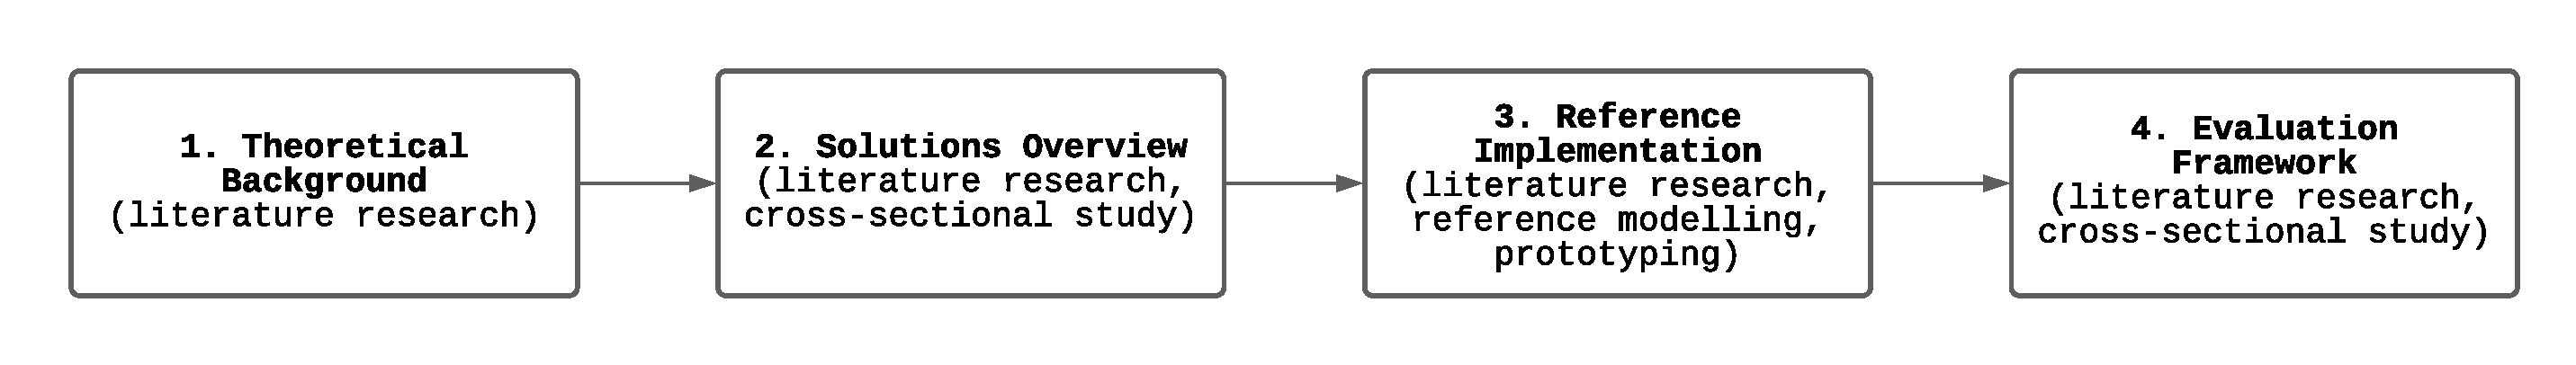
\includegraphics[width=\textwidth]{../img/1_approach_h.eps}}
        \caption{Research Approach}
        \label{figure: approach}
    \end{figure}
	
    For this purpose, various methods of business and information systems engineering according to \cite{wilde_forschungsmethoden_2007} are applied. Through a literature research, an overview of existing papers and books is created, which on the one hand serves for building a theoretical foundation, but also represents the basis for all other steps. 
    
    To find the literature, keywords such as “Self-sovereign Identity” and the following complex query based on \cite{van_bokkem_self-sovereign_2019} were used at Google Scholar:
    \begin{verbatim}
    ("Self-sovereign identity" OR "Self sovereign identity ") 
    OR ( 
        ("block−chain" OR "blockchain") AND ("identity management")
        AND ("solution" OR "implementation" OR "review" OR "survey")            
        AND ("verifiable credentials" OR "decentralized identifiers")
    )
    \end{verbatim}
    Furthermore, the method of cross-sectional studies, mainly in the form of expert questionnaires, is used. A clearly defined set of questions is used to validate the solutions overview, but also to identify evaluation criteria for the evaluation framework. More details on the selection of experts and the questions are described in section X.X. For the creation of the reference implementation, the methods of reference modelling and prototyping are used. In combination, they allow the development of a software prototype that represents a particular problem in a simplified way and whose analysis can contribute to the discovery of new knowledge. This is especially interesting for the development of the evaluation framework. Moreover, it should also be noted that this thesis follows the general idea of generating real-world artefacts defined by \cite{hevner_three_2007} as part of design science research.
    
    To conclude the methodology, a combination of research approach and applied methods defined previously is reflected in the following research questions: 
    
    % Might have to change them up?
    \begin{enumerate}
      \item What libraries, platforms, or SDKs are available for implementing Verifiable Credentials?
      \item Which SDKs do experts from the field recommend using?
      \item Which criteria for evaluating Verifiable Credential SDKs can be derived after developing a reference implementation?
    \end{enumerate}